\chapterimage{orange2.jpg} % Chapter heading image
\chapterspaceabove{6.75cm} % Whitespace from the top of the page to the chapter title on chapter pages
\chapterspacebelow{7.25cm} % Amount of vertical whitespace from the top margin to the start of the text on chapter pages

\chapter{Input-to-State Stability}\index{Input-to-State Stability}

\section{Overview}\index{Overview}
We have studied two main types of stability: \textbf{Lyapunov stability}, which concerns equilibrium points of unforced state-space systems, and \textbf{input-output stability}, which focuses only on the relation between inputs and outputs. These two concepts lie at opposite ends---one emphasizes internal dynamics, while the other ignores them. To connect these perspectives, we introduce the idea of \textbf{input-to-state stability (ISS)}. ISS considers systems with inputs and analyzes stability in terms of both the state and the input’s effect.

\section{Motivation}\index{Motivation}

We consider the nonlinear system
\begin{equation}
\dot{x} = f(x,u),
\end{equation}
where $f(x,u)$ is locally Lipschitz in $x$ and $u$. This guarantees local existence and uniqueness of solutions.  

\noindent
We assume that the unforced system
\begin{equation}
\dot{x} = f(x,0)
\end{equation}
has a uniformly asymptotically stable equilibrium at $x=0$. 

\noindent
The central question is: \emph{if the origin is asymptotically stable when $u=0$, what happens when $u \neq 0$?} Specifically:
\begin{enumerate}
    \item \textbf{If $\lim_{t \to \infty} u(t) = 0$, does it follow that $\lim_{t \to \infty} x(t) = 0$?}
    \item \textbf{If $u(t)$ is bounded, does this imply that $x(t)$ is also bounded?}
\end{enumerate}

\noindent
For linear time-invariant (LTI) systems, the answer is \emph{yes}. Given
\begin{equation}
\dot{x} = Ax + Bu,
\end{equation}
the solution is
\begin{equation}
x(t) = e^{At}x_0 + \int_0^t e^{A(t-\tau)}Bu(\tau)\, d\tau.
\end{equation}
If $A$ is stable ($\text{Re}(\lambda_i(A))<0$), then bounded inputs lead to bounded states, and vanishing inputs imply $x(t)\to 0$. 

\noindent
However, in the nonlinear case, this property \emph{does not always hold}.  

\begin{example}[Nonlinear System with Bounded Input]
Consider the nonlinear system
\begin{equation}
    \dot{x} = -x + (x+x^3)u.
\end{equation}

\textbf{Case 1: Unforced system ($u=0$).}  
The dynamics reduce to
\begin{equation}
    \dot{x} = -x,
\end{equation}
which has the equilibrium $x=0$. Since solutions decay exponentially to zero, the origin is \textbf{asymptotically stable}.  

\textbf{Case 2: Forced system with constant input ($u(t)=1$).}  
The dynamics become
\begin{equation}
    \dot{x} = x^3.
\end{equation}
For any initial condition $x(0)\neq 0$, the trajectory grows unbounded in finite time:
\begin{equation}
    x(t) = \frac{x(0)}{\sqrt{1 - 2t\,x(0)^2}}.
\end{equation}

Thus, even though the unforced system is asymptotically stable, the forced system with bounded input leads to unbounded trajectories.  

\textbf{Conclusion:} This example shows that stability properties of linear systems (where bounded inputs imply bounded states) do not necessarily extend to nonlinear systems.
\end{example}


This shows that nonlinear systems can behave very differently from LTI systems, motivating the study of \textbf{Input-to-State Stability (ISS)}.

\section{Definitions}\index{Definitions}

\begin{definition}[Class $\mathcal{K}$ function]
A continuous function $\alpha:[0,\infty)\to[0,\infty)$ is said to be of 
\emph{class $\mathcal{K}$} if
\begin{enumerate}
    \item $\alpha(0)=0$, and
    \item $\alpha$ is strictly increasing, i.e., $\alpha(s_1)<\alpha(s_2)$ whenever $s_1<s_2$.
\end{enumerate}
If in addition $\alpha(s)\to\infty$ as $s\to\infty$, then $\alpha$ is called a 
\emph{class $\mathcal{K}_\infty$} function.
\end{definition}

\begin{definition}[Class $\mathcal{KL}$ function]
A continuous function $\beta:[0,\infty)\times [0,\infty)\to[0,\infty)$ is said to be of
\emph{class $\mathcal{KL}$} if
\begin{enumerate}
    \item for each fixed $t\ge 0$, the mapping $r\mapsto \beta(r,t)$ belongs to class $\mathcal{K}$,
    \item for each fixed $r\ge 0$, the mapping $t\mapsto \beta(r,t)$ is decreasing and satisfies
    \[
    \lim_{t\to\infty}\beta(r,t)=0.
    \]
\end{enumerate}
\end{definition}

\begin{example}
\begin{itemize}
    \item $\alpha(s) = ks$ with $k>0$ is a class $\mathcal{K}_\infty$ function.
    \item $\alpha(s) = \tanh(s)$ is a class $\mathcal{K}$ function but not $\mathcal{K}_\infty$.
    \item $\beta(r,t) = r e^{-\lambda t}$, with $\lambda>0$, is a class $\mathcal{KL}$ function.
\end{itemize}
\end{example}

\begin{definition}[Input-to-State Stability (ISS)]
Consider the nonlinear system
\begin{equation}
    \dot{x} = f(x,u).
\end{equation}
The system is said to be \emph{input-to-state stable (ISS)} if there exist functions 
$\beta \in \mathcal{KL}$ and $\gamma \in \mathcal{K}$ such that, for all $t \geq 0$,
\begin{equation}
    \|x(t)\| \;\leq\; \beta(\|x_0\|,t) \;+\; \gamma\!\left(\sup_{0\le \tau \le t}\|u(\tau)\|\right),
\end{equation}
for every initial condition $x(0)=x_0$ and every bounded input $u(\cdot)$.  
\end{definition}

\begin{remark}
The inequality above splits the effect of the initial state and the input:
\begin{itemize}
    \item If the input is zero, $u(t)\equiv 0$, then the solution satisfies
    \[
    \|x(t)\| \leq \beta(\|x_0\|,t),
    \]
    which shows that the origin is \emph{uniformly asymptotically stable}.
    \item If the input is bounded, say $\|u(t)\|\leq b$ for all $t$, then after some time the state $x(t)$ enters and stays inside a ball of radius $\gamma(b)$. This radius is called the \emph{ultimate bound}.
\end{itemize}
\end{remark}

\begin{definition}[ISS Lyapunov Function]
A smooth function $V:D \subseteq \mathbb{R}^n \to \mathbb{R}_{\ge 0}$ is an \emph{ISS Lyapunov function} if there exist class $\mathcal{K}_\infty$ functions $\alpha_1, \alpha_2, \alpha_3$ and a class $\mathcal{K}$ function $\gamma$ such that:
\begin{align}
    \alpha_1(\|x\|) \;\leq\; V(x) \;\leq\; \alpha_2(\|x\|), \label{eq:iss-v-bounds}\\[6pt]
    \dot V(x,u) \;\leq\; -\alpha_3(\|x\|), 
    \quad \text{whenever } \|x\| \;\geq\; \gamma(\|u\|). \label{eq:iss-v-decay}
\end{align}
\end{definition}

\begin{remark}
Condition \eqref{eq:iss-v-bounds} guarantees that $V$ behaves like a measure of the state size: it is positive definite and radially unbounded. In other words, $V(x)\ge 0$ for all $x$, and $V(x)=0$ only at $x=0$.
\end{remark}

\begin{remark}
Condition \eqref{eq:iss-v-decay} means that whenever the state is outside a ball whose radius depends on the input size, the Lyapunov function strictly decreases. 
Thus, large states are always forced to shrink, which ensures that trajectories remain bounded and eventually approach a neighborhood of the origin whose size is proportional to the input bound.
\end{remark}

\section{Input-to-State Stability (ISS) Theorems}\index{ISS Theorems}

\begin{theorem}[Local ISS Theorem]
Consider the nonlinear system
\begin{equation}
    \dot{x} = f(x,u),
\end{equation}
and let $V:D\to\mathbb{R}_{\ge 0}$ be an ISS Lyapunov function. Then the system is 
\emph{locally input-to-state stable}, meaning that there exist class $\mathcal{KL}$ 
and class $\mathcal{K}$ functions $\beta$ and $\gamma$ such that
\begin{equation}
    \|x(t)\| \;\leq\; \beta(\|x_0\|,t) \;+\; 
    \gamma\!\Big(\sup_{0\le \tau \le t}\|u(\tau)\|\Big),
\end{equation}
for all initial conditions $x_0$ in a neighborhood of the origin and for all bounded 
inputs $u(\cdot)$.  
\end{theorem}

\begin{theorem}[Global ISS Theorem]
If the same conditions hold globally with $D = \mathbb{R}^n$, $Du = \mathbb{R}^m$, 
and $\alpha_i \in \mathcal{K}_\infty$, then the system is 
\emph{globally input-to-state stable}.  

This means that for any initial state and any bounded input, the trajectories satisfy
\begin{equation}
\|x(t)\| \;\leq\; \beta(\|x_0\|,t) \;+\; 
\gamma\!\Big(\sup_{0\le \tau \le t}\|u(\tau)\|\Big), 
\qquad \forall t\ge 0.
\end{equation}
\end{theorem}

\begin{remark}
ISS Lyapunov functions capture two essential properties:
\begin{itemize}
    \item When $u(t)\equiv 0$, the inequality reduces to 
    $\|x(t)\|\leq \beta(\|x_0\|,t)$, which shows that the origin is globally asymptotically stable.
    \item For bounded inputs, the state remains bounded and eventually enters a ball of radius $\gamma(\|u\|)$, called the \emph{ultimate bound}.
\end{itemize}
\end{remark}

\subsection{Examples of ISS}\index{ISS Theorems!Examples of ISS}

\begin{example}[Cubic stabilization with additive input]
Consider 
\begin{equation}
    \dot{x} = -a x^3 + u, \qquad a>0.
\end{equation}
Take the candidate Lyapunov function
\begin{equation}
    V(x) = \tfrac{1}{2}x^2.
\end{equation}
Compute its time derivative:
\begin{equation}
    \dot V(x) = \frac{d}{dt}\!\left(\tfrac{1}{2}x^2\right) = x\dot x,
\end{equation}
\begin{equation}
    \dot V(x) = x(-a x^3 + u) = -a x^4 + x u.
\end{equation}
Bounding the input term:
\begin{equation}
    \dot V(x) \le -a x^4 + |x|\,|u|.
\end{equation}
For $x\neq 0$, divide by $|x|$:
\begin{equation}
    a|x|^3 > |u| \quad \Longleftrightarrow \quad |x| > \left(\frac{|u|}{a}\right)^{1/3}.
\end{equation}
Thus $\dot V<0$ whenever $|x|>(|u|/a)^{1/3}$, proving global ISS with 
\(\gamma(\|u\|)\propto \|u\|^{1/3}\).
\end{example}

\begin{example}[Multiplicative input]
Consider
\begin{equation}
    \dot{x} = -a x^3 + x^2 u, \qquad a>0.
\end{equation}
Choose
\begin{equation}
    V(x)=\tfrac{1}{2}x^2.
\end{equation}
Then
\begin{equation}
    \dot V = x\dot x = x(-a x^3 + x^2 u) = -a x^4 + x^3 u.
\end{equation}
Bounding the input term:
\begin{equation}
    \dot V \le -a x^4 + |x|^3 |u|.
\end{equation}
For $x\neq 0$, divide by $|x|^3$:
\begin{equation}
    a|x| > |u| \quad \Longleftrightarrow \quad |x| > \frac{|u|}{a}.
\end{equation}
Thus $\dot V<0$ whenever $|x| > \dfrac{|u|}{a}$, showing global ISS.
\end{example}

\begin{example}[Input with state-dependent gain]
Consider
\begin{equation}
    \dot{x} = -a x^3 + x(1+x^2)u, \qquad a>0.
\end{equation}
Take
\begin{equation}
    V(x)=\tfrac{1}{2}x^2.
\end{equation}
Then
\begin{equation}
    \dot V = x\dot x = x(-a x^3 + x(1+x^2)u),
\end{equation}
\begin{equation}
    \dot V = -a x^4 + x^2(1+x^2)u.
\end{equation}
Bounding the input term:
\begin{equation}
    \dot V \le -a x^4 + |x|^2(1+x^2)\,|u|.
\end{equation}
For $x\neq 0$, divide by $|x|^2$:
\begin{equation}
    a x^2 > (1+x^2)|u|.
\end{equation}
Rearranging:
\begin{equation}
    x^2(a-|u|) > |u|.
\end{equation}
Thus, if $a>|u|$, a sufficient condition for $\dot V<0$ is
\begin{equation}
    |x| > \sqrt{\frac{|u|}{a-|u|}}.
\end{equation}
Hence, for sufficiently large states, the damping dominates and the system is ISS, 
with bounds depending on both input and parameters.
\end{example}


\section{Input-to-State Stability Revisited}\index{ISS Revisited}

\begin{definition}[Dissipation inequality / ISS pair]
A pair of continuous class $\mathcal{K}$ functions $(\alpha_3,\sigma)$ is called an 
\emph{ISS pair} for the system $\dot x=f(x,u)$ if there exists a continuous function 
$V:D\to\mathbb{R}_{\ge 0}$ and class $\mathcal{K}_\infty$ functions 
$\alpha_1,\alpha_2$ such that
\begin{equation}
    \alpha_1(\|x\|)\le V(x)\le \alpha_2(\|x\|), \label{eq:Vbounds}
\end{equation}
and
\begin{equation}
    \nabla V(x)\cdot f(x,u) \le -\alpha_3(\|x\|) + \sigma(\|u\|),
    \label{eq:dissipation}
\end{equation}
for all $(x,u)\in D\times D_u$. Equation \eqref{eq:dissipation} is called the 
\emph{dissipation inequality}.
\end{definition}

\begin{theorem}[ISS equivalence]
The system $\dot x=f(x,u)$ is input-to-state stable (ISS) on $D$ if and only if there 
exists a continuous function $V$ and class $\mathcal{K}$ functions 
$\alpha_1,\alpha_2,\alpha_3,\sigma$ satisfying \eqref{eq:Vbounds}--\eqref{eq:dissipation}.
\end{theorem}

\begin{remark}
The dissipation inequality separates the natural decay of the system, 
$-\alpha_3(\|x\|)$, from the disturbance caused by the input, $\sigma(\|u\|)$. 
Large states always decrease unless sustained by input energy, and bounded inputs 
determine the ultimate bound around the origin.
\end{remark}

\begin{theorem}[Local ISS via classical Lyapunov]
If the origin of the unforced system $\dot x=f(x,0)$ is asymptotically stable and 
$f$ is continuously differentiable, then the system is locally ISS.
\end{theorem}

\begin{remark}
For sufficiently small initial states and inputs, trajectories remain bounded near 
the origin. This captures a local form of input-to-state stability.
\end{remark}

\begin{theorem}[Global ISS via classical Lyapunov]
If the origin of the unforced system $\dot x=f(x,0)$ is globally exponentially stable, 
$f$ is continuously differentiable, and globally Lipschitz, then the system is globally ISS.
\end{theorem}

\begin{remark}
Global exponential stability ensures that any bounded input produces a bounded state, 
valid for all initial conditions. This establishes global ISS.
\end{remark}

\begin{theorem}[Characterization via ISS Lyapunov functions]
A continuous function $V:D\to\mathbb{R}_{\ge 0}$ is an ISS Lyapunov function if and 
only if there exist class $\mathcal{K}$ functions $\alpha_1,\alpha_2,\alpha_3,\sigma$ such that
\begin{align}
    \alpha_1(\|x\|) &\le V(x) \le \alpha_2(\|x\|), \\
    \nabla V(x) \cdot f(x,u) &\le -\alpha_3(\|x\|) + \sigma(\|u\|),
    \quad x\in D,\, u\in D_u.
\end{align}
\end{theorem}

\begin{remark}
This result formalizes ISS in terms of Lyapunov functions. 
It shows that the state always decreases when sufficiently large, 
except for the influence of inputs.
\end{remark}

\subsection{Constructive results: modifying ISS pairs}\index{ISS Revisited!Constructive results: modifying ISS pairs}

\begin{definition}[Big-O notation]
Let $f,g:[0,\infty)\to\mathbb{R}$ be functions.  

\begin{itemize}
    \item We write 
    \[
    f(r) = O(g(r)) \quad \text{as } r \to \infty
    \]
    if there exist constants $C>0$ and $r_0 \ge 0$ such that
    \[
    |f(r)| \le C\,|g(r)| \qquad \text{for all } r \ge r_0.
    \]
    \item We write 
    \[
    f(r) = O(g(r)) \quad \text{as } r \to 0^+
    \]
    if there exist constants $C>0$ and $\delta > 0$ such that
    \[
    |f(r)| \le C\,|g(r)| \qquad \text{for all } 0<r \le \delta.
    \]
\end{itemize}
\end{definition}

\begin{theorem}[Adjustment at infinity]
Let $(\alpha_3,\sigma)$ be an ISS pair and $\rho\in\mathcal{K}_\infty$ satisfy 
$\sigma(r) = O(\rho(r))$ as $r\to\infty$. Then, there exists 
$\tilde\sigma\in\mathcal{K}_\infty$ such that $(\alpha_3,\tilde\sigma)$ is also an ISS pair.
\end{theorem}

\begin{theorem}[Adjustment near zero]
Let $(\alpha_3,\sigma)$ be an ISS pair and $\rho\in\mathcal{K}_\infty$ satisfy 
$\alpha_3(r) = O(\rho(r))$ as $r\to 0^+$. Then, there exists 
$\tilde\alpha_3\in\mathcal{K}_\infty$ such that $(\tilde\alpha_3,\sigma)$ 
is also an ISS pair.
\end{theorem}

\begin{remark}
These constructive results show that different ISS pairs can describe the same system. 
They provide flexibility in adjusting the decay rate and input gain either near the origin 
or for large signals, which is useful in applications such as small-gain analysis.
\end{remark}

\section{Cascade-Connected Systems}\index{Cascade-Connected Systems}

\begin{figure}[h]
\centering
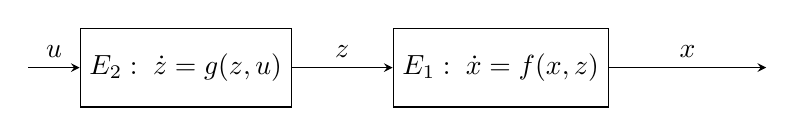
\begin{tikzpicture}[scale=1.0, node distance=4cm, >=stealth]
\node[draw, rectangle, minimum width=2cm, minimum height=1cm] (E2) {$E_2:\;\dot z=g(z,u)$};
\node[draw, rectangle, minimum width=2cm, minimum height=1cm, right of=E2] (E1) {$E_1:\;\dot x=f(x,z)$};
\draw[->] (-2,0) -- (E2.west) node[midway, above] {$u$};
\draw[->] (E2.east) -- (E1.west) node[midway, above] {$z$};
\draw[->] (E1.east) -- +(2,0) node[midway, above] {$x$};
\end{tikzpicture}
\caption{Cascade connection of two ISS systems: the state $z$ of $E_2$ acts as the input to $E_1$.}
\label{fig:cascade}
\end{figure}

Consider the cascade interconnection in Figure~\ref{fig:cascade}, where 
\begin{align}
E_1: \quad & \dot{x} = f(x,z), \\
E_2: \quad & \dot{z} = g(z,u),
\end{align}
and the state $z$ of $E_2$ serves as the input to $E_1$. 

\subsection{ISS properties of cascades}\index{Cascade-Connected Systems!ISS properties of cascades}

\begin{proposition}[Alternative ISS pairs]
Suppose $E_1$ and $E_2$ are ISS with ISS pairs $[\alpha_1,\sigma_1]$ and 
$[\alpha_2,\sigma_2]$, respectively. That is, there exist positive definite Lyapunov 
functions $V_1,V_2$ such that
\begin{align}
\nabla V_1 \cdot f(x,z) &\le -\alpha_1(\|x\|) + \sigma_1(\|z\|), \\
\nabla V_2 \cdot g(z,u) &\le -\alpha_2(\|z\|) + \sigma_2(\|u\|).
\end{align}
Then there exist alternative ISS pairs $[\tilde{\alpha}_1,\tilde{\sigma}_1]$ and 
$[\tilde{\alpha}_2,\tilde{\sigma}_2]$ for $E_1$ and $E_2$.
\end{proposition}

\begin{remark}
This flexibility in choosing ISS pairs is important when analyzing interconnected systems: 
it allows the bounds of one subsystem to be reshaped to fit the stability proof for the cascade.
\end{remark}

\begin{theorem}[Global ISS for cascades]
If both $E_1$ and $E_2$ are ISS, then the composite cascade system
\[
(x,z) \mapsto (f(x,z),\, g(z,u))
\]
is also ISS. A valid ISS Lyapunov function for the cascade is
\begin{equation}
    V(x,z) = V_1(x) + V_2(z),
\end{equation}
which satisfies
\begin{equation}
\nabla V \cdot 
\begin{bmatrix} f(x,z) \\ g(z,u) \end{bmatrix}
\;\le\; -\alpha_1(\|x\|) - \alpha_2(\|z\|) + \sigma_2(\|u\|).
\end{equation}
\end{theorem}

\begin{remark}
The cascade inherits ISS from its components. The joint Lyapunov function $V(x,z)$ 
decreases whenever $(x,z)$ is large relative to the input, ensuring boundedness and 
ultimate stability in terms of $u$.
\end{remark}

\begin{theorem}[Local ISS for cascades]
If $E_1$ and $E_2$ are locally ISS, then the cascade system is locally ISS.
\end{theorem}

\begin{remark}
This ensures that for small initial conditions and small inputs, the trajectories 
remain bounded and close to the origin.
\end{remark}

\subsection{Asymptotic stability results}\index{Cascade-Connected Systems!Asymptotic stability results}

\begin{corollary}[Local asymptotic stability of cascades]
Suppose:
\begin{itemize}
    \item The subsystem $E_1$ is \emph{locally ISS} with respect to its input $z$, and
    \item The origin of $E_2$ is \emph{asymptotically stable}.
\end{itemize}
Then the equilibrium point $(x,z)=(0,0)$ of the cascade system is \emph{locally asymptotically stable}.
\end{corollary}

\begin{corollary}[Global asymptotic stability of cascades]
Suppose:
\begin{itemize}
    \item The subsystem $E_1$ is \emph{ISS} (globally), and
    \item The origin of $E_2$ is \emph{globally asymptotically stable}.
\end{itemize}
Then the equilibrium point $(x,z)=(0,0)$ of the cascade system is 
\emph{globally asymptotically stable}.
\end{corollary}

\begin{remark}
These corollaries illustrate a simple principle:
\begin{itemize}
    \item The downstream subsystem $E_2$ acts like a \emph{filter} between the input $u$ 
    and the upstream subsystem $E_1$.
    \item If $E_2$ settles to the origin (locally or globally), then its state $z(t)$ 
    eventually becomes small (or vanishes).
    \item Since $E_1$ is ISS with respect to $z$, a vanishing input $z(t)$ implies that $x(t)$ 
    also converges to zero.
\end{itemize}
Therefore, the overall cascade $(x,z)$ converges to the origin, with the stability 
(local or global) determined by the properties of $E_2$.
\end{remark}



